%
% teil2.tex
%
% (c) 2023 Vincent Haufe, Hochschule Rapperswil
%
% !TEX root = ../../buch.tex
% !TEX encoding = UTF-8

\section{Konstruktion der Mellin-Transformation
\label{mellin:section:teil2}}
\rhead{Mellin-Transformation}
Wie schon bemerkt, sind wir bei diesem Problem mit der multiplikativen 
Gruppe der positiven reellen Zahlen $(\mathbb{R^+},\cdot)$ konfrontiert 
\footnote{Eine ausführliche Beschreibung dessen, was in diesem Abschnitt 
folgt, findet sich im Kapitel \ref{buch:chapter:gruppen} diese Buches}.
\begin{definition}
    Eine Gruppe setzt sich aus einer \textbf{Menge} und einer 
    \textbf{Verknüpfung} zusammen. 
    Elemente aus der Menge können über die Verknüpfung miteinander 
    verrechnet werden, müssen aber stets wieder Elemente der Menge bilden.
\end{definition}
Diese Information ist der Startpunkt auf der Suche nach einer 
Integraltransformation die unser Problem lösen kann.
Die Gelfandtheorie ist die verallgemeinerte Theorie der Fourieranalyse und 
beschreibt die notwendigen Bausteine einer solchen.
Zum einen sind \textbf{Analysefunktionen} zu bestimmen, welche die 
Gruppenoperation in die Multiplikation überführt und gewisse 
Orthogonalitätsbedingungen erfüllen. 
Des Weiteren muss das \textbf{Skalarprodukt} auf die multiplikative Gruppe 
angepasst werden, mit dem die Integraltransformation durchgeführt werden 
soll.
Aus Gruppe, Analysefunktionen und Skalarprodukt folgt dann 
\footnote{für kommutative Lie-Gruppen} die entsprechende Transformation.
% Diese Bedingungen mögen dem Ingenieur auf den ersten Blick etwas ominös und sehr abstrahiert erscheinen, was aber auch der im Sinne 
% einer verallgemeinerten Theorie ist.
% Im Folgenden soll konkret gezeigt werden, wie sich also mithilfe dieser Theorie



% Prinzipien:

% -Gruppe 
% -Analysefunktionen sind Homomorphismen und orthogonal zueinander: h (Eigenfunktionen (Differential)operator?)
% -Skalarprodukt (Integral)
% -Analyse <h,f> = Gf(h)
% -Faltung: Integral über ganze Gruppe mit Gruppenoperation
% -Faltungsformel: Aus Faltung wird Produkt
% -zulässige h bilden duale Gruppe -> Plancherel


\subsection{Analysefunktionen der Mellin-Transformation
\label{mellin:subsection:analysefunktionen}}

Unser Ziel ist es, die für unser Registrierungsproblem neu definierte 
Kreuzkorrelation mithilfe einer Integraltransformation in 
einfache Multiplikation der transformierten Funktionen zu verwandeln.
Dafür braucht es spezielle Funktionen, sogenannte Homomorphismen, welche 
die Gruppenoperation in die Multiplikation überführen können. 
\begin{satz}
    \label{buch:papers:mellin:teil2:satz:hom}
    Eine (kommutative?) Integraltransformation enthält das Faltungstheorem.
    Dafür braucht es Funktionen, welche die Gruppenoperation in eine 
    \textbf{Multiplikation} überführt. 
    \[
        f(x \diamond y) 
        = f(x) \cdot f(y)
        ,
    \]
    wobei $\diamond$ der Gruppenoperation enstpricht.
\end{satz}
Dies gilt sowohl für die Gruppenoperationen der Gruppe im Ortsraum als auch 
für die Gruppenoperation der dualen Gruppe im Bildraum der Transformation.
Mit dem Konzept der dualen Gruppe werden wir uns am Ende des Abschnitts 
nochmals genauer befassen, fürs Erste konzentrieren wir uns auf die 
multiplikative Gruppe in $\mathbb{R^+}$, welche relevant für unsere 
skalierten Funktionen ist, also im Ortsraum.
\medskip

Bei der Fouriertransformation, dessen Gruppenoperation die Additon ist, 
müssen die Analysefunktionen also die Gleichung 
\begin{equation}
    f(x + y) 
    = f(x) \cdot f(y)
    \label{mellin:hom1}
\end{equation}
erfüllen. 
Die Funktion, die diese Eigenschaft besitzt ist natürlich die 
Exponentialfunktionen, denn 
\begin{equation}
    e^{x + y} 
    = e^x \cdot e^y
    ,
    \label{mellin:exp}
\end{equation}
und somit die bekannte Analysefunktion der Fouriertransformation.
In der Fortsetzung bedeutet das für die neue Transformation, dass dessen 
Analysefunktionen die Gleichung
\begin{equation}
    f(x \cdot y) 
    = f(x) \cdot f(y)
    \label{mellin:hom2}
\end{equation}
erfüllen müssen.
Erfüllt wird die Gleichung durch jede Potenzfunktion $h(x) = x^{-z}$ für 
beliebige $z \in \mathbb{C}$ \footnote{das Minus vor dem $z$ ist bezüglich 
der Homomorphismuseigenschaft unbedeutend, muss aber aus demselben Grund 
wie bei der Fouriertransformation ($e^{-j\omega t}$) enthalten sein, auf 
den hier aber nicht eingegangen werden soll}
\begin{equation}
    h(x \cdot y) 
    = (x \cdot y)^{z} = x^{z} \cdot y^{z}
    ,
\end{equation}
% denn Potenzen lassen sich bekanntlich beliebig zusammenfassen so wie
% \begin{equation}
%     (a \cdot b)^2 = a^2 \cdot b^2 \left(\frac{a}{b}\right)^2  = \frac{a^2}{b^2} 
% \end{equation}
Unsere Analysefunktionen müssen also vom Typ Potenzfunktion sein.
% Zudem muss, damit eine Transformation existiert, sichergestellt sein, dass die Integrale der Transformation konvergieren.
% Deshalb 
% Die komplexe Exponentialfunktion $e^{j\omega_l t}$ ist orthogonal zu $e^{j\omega_k t}$, sofern $\omega_l \neq \omega_k$, da diese 
% immer ein Skalarprodukt gleich Null haben wie sich leicht zeigen lässt
% \begin{proof}
%     \begin{align*}
%         \langle h_l,h_k \rangle &= \int_\mathbb{R} e^{j\omega_l t} \cdot e^{-j\omega_k t}\,dt \\
%         &= \int_\mathbb{R} e^{j(\omega_l - \omega_l) t}\,dt \\
%         &= \int_\mathbb{R} e^{j\omega_l-k t}\,dt = 0 \vert \omega_l \neq \omega_k 
%     \end{align*}
%     Da die komplexe Exponentialfunktion periodisch ist.
% \end{proof}
% Bei den komplexen Exponentialfunktionen der Fouriertransformation ist dies auch intuitiv, da dahinter die Sinus- und 
% Cosinusschwingungen unterschiedlicher Frequenzen stehen, in die eine Funktion zerlegt werden kann.


\subsection{Skalarprodukt der Mellin-Transformation
\label{mellin:subsection:skalarprodukt}}
Die Entdeckung der Fourierreihen brachte die Notwendigkeit mit sich, den 
Riemannschen Integralbegriff \footnote{Siehe auch Kapitel 
\ref{buch:skalarprodukt:section:funktionenraeume}} zu überdenken und zu 
präzisieren.
Dafür wurde vor allem die aufkommende Masstheorie angewendet.
Relevant ist dabei nun, dass wir für unser Integral und somit Skalarprodukt 
mit welchem wir die Transformation durchführen wollen, 
mit einem \textbf{Mass}\footnote{in diesem Kontext genauer: ein Haar-Mass} 
ausstatten. 
Damit gelingt es uns, das Integral 
\emph{invariant bezüglich der Gruppenoperation} zu machen, was für den 
Erfolg der Fouriertheorie zwingend nötig ist. 
\begin{satz}
    \label{buch:papers:mellin:teil2:satz:int}
    Das Integral, mit dem eine Integraltransformation durchgeführt wird, 
    muss \textbf{invariant bezüglich der Gruppenoperation} der Gruppe 
    der zu transformierenden Funktionen sein.
    \[
        \int_\mathbb{G} f(x)\,\mathrm{d}x 
        = \int_\mathbb{G} f(x \diamond x_0)\,\mathrm{d}x
    \]
\end{satz}
Invariant bezüglich der Gruppenoperation bedeutet, dass sich das Integral 
über den gesamten Definitionsbereich der Gruppe nicht ändert, wenn das 
Argument der zu integrierenden Funktion ``verschoben'' wird. 
Das gewöhnliche Integral der Fouriertransformation erfüllt diese 
Eigenschaft 
\begin{equation}
    \int_\mathbb{R} f(x)\,\mathrm{d}x 
    = \int_\mathbb{R} f(x + x_0)\,\mathrm{d}x
\end{equation}
da hier ja von $-\infty$ bis $+\infty$ integriert wird und somit eine nur 
endlich verschobene Funktion stets vollständig abmisst.
Verschoben meint in diesem Sinne aber Verschiebung mit der Gruppenoperation, 
was bei Fourier also ein ``+'' war, wird bei unserer neuen Transformation 
zu einem ``$\cdot$'', das heisst zu einer Streckung des Arguments. 
Es wird schnell klar, dass das herkömmliche Integral eben \emph{nicht} 
invariant bezüglich dieser Streckung ist und allgemein gilt 
\begin{equation}
    \int_\mathbb{R^+} 
    f(x)\,\mathrm{d}x \neq \int_\mathbb{R^+} f(s \cdot x)\,\mathrm{d}x
\end{equation}
da, einfach gesagt, eine Streckung der x-Achse die Funktion und somit deren
 Flächeninhalt auseinderzieht.
Es braucht nun also eine Anpassung, um diese Veränderung des Flächeninhalts 
zu kompensieren.
Das kann überraschend einfach mithilfe einer Division durch die Variable 
des Arguments $x$ erreicht werden, was auch sehr einfach gezeigt werden 
kann.
\begin{proof}[Beweis]
    Zu beweisen ist die folgende Gleichung:
    \[
        \int_\mathbb{R^+} f(s \cdot x)\,\frac{\mathrm{d}x}{x} 
        = \int_\mathbb{R^+} f(x)\,\frac{\mathrm{d}x}{x}
    \]
    Eine Substitution von $s \cdot x$ mit $u$
    \begin{align*}
        u &= sx \\
        x &= \frac{u}{s} \\
        \mathrm{d}x &= \frac{1}{s} \mathrm{d}u
    \end{align*}
    führt auf
    \[
        \int_\mathbb{R^+} f(sx) \cdot x^{-1}\,\mathrm{d}x 
        = \int_\mathbb{R^+} f(u) \cdot \frac{s}{u} \frac{1}{s}\,\mathrm{d}u
        = \int_\mathbb{R^+} f(u)\,\frac{\mathrm{d}u}{u}
    \]
    Was beweist, dass sich der Faktor $s$ durch das zusätzliche Mass 
    $x^{-1}$ herauskürzt. 
\end{proof}
Eine Intuition für diesen Umstand liefert auch ein Beispiel.
\begin{beispiel}
Man betrachte die Funktion 
\[
f(x) 
= 
\begin{cases}
    x^3 &\qquad 0\leq x\leq 1\\
    0 &\qquad \text{sonst}
\end{cases}
\]
% to do
\end{beispiel}
Das für die Multiplikation als Gruppenoperation modifizierte Integral ist 
somit
\begin{equation}
    \int_\mathbb{R^+} f(x)\,\frac{\mathrm{d}x}{x}
    ,
\end{equation}
und das Skalarprodukt mit dem die Transformation erfolgt
\begin{equation}
    \langle f,g \rangle 
    = \int_\mathbb{R^+} \overline{f(x)} \cdot g(x) \,\frac{\mathrm{d}x}{x}
    .
\end{equation}
% Are you sure?


\subsection{Korrelation und Faltung auf $\mathbb{R^+}$
\label{mellin:subsection:faltung}}
Wir haben nun alle essenziellen Bausteine beisammen um die gesuchte 
Transformation zu formulieren: grundlegende Gruppe, Analysefunktionen 
und Skalarprodukt.
Das Rezept dafür lautet nun wie folgt. Es wird das für die Gruppe neu 
definierte Skalarprodukt der Analysefunktion $h(x)$ mit der zu 
transformierenden Funktion $f(x)$ gebildet.
\begin{equation}
    \langle h,f \rangle 
    = \int\limits_{0}^{\infty} x^{z} f(x) \,\frac{\mathrm{d}x}{x}
\end{equation}
eine kleine Umformung führt zu einer kompakten Formel der 
\emph{Mellin-Transformation}
\begin{equation}
    \mathcal{M}\{f \}(z) 
    = \int\limits_{0}^{\infty} x^{z-1} f(x) \,\mathrm{d}x 
    \qquad\text{für $z \in \mathbb{C}$}
    \label{mellin:mellin}
\end{equation}
Dies ist die allgemeinste Form der Mellin-Transformation. 
Wenn man aber die komplexe Zahl $z = \delta + ju$ auf ihren Imaginärteil 
beschränkt $\operatorname{Re}(z) = \delta = 0$ erhält man die Formel
\begin{equation}
    \mathcal{M}\{f \}(u) 
    = \int\limits_{0}^{\infty} x^{ju-1} f(x) \,\mathrm{d}x 
    \qquad\text{für $u \in \mathbb{R}$}
    ,
    \label{mellin:mellinu}
\end{equation}
die sich noch als nützlich und intuitiv erweisen wird.

Ebenfalls lassen sich die Korrelation sowie die Faltung über die 
Gruppenoperation und das modifizierte Skalarprodukt bestimmen:
\begin{equation}
    (f \star g)(\sigma ) 
    = \int_\mathbb{R^+} 
    f(x) \cdot g(\sigma ^{-1} \cdot x)\,\frac{\mathrm{d}x}{x}
    \label{mellin:kreuzkorrelation*}
\end{equation}
\begin{equation}
    (f \ast g)(x) 
    = \int_\mathbb{R^+} 
    f(y) \cdot g(x \cdot y^{-1})\,\frac{\mathrm{d}y}{y} 
\end{equation}
Damit erhalten wir von der Gelfandtheorie zum krönenden Abschluss das 
Faltungstheorem
\begin{equation}
    \mathcal{M}\left\{f \ast g\right\} 
    = \mathcal{M}\left\{f\right\} \cdot \mathcal{M}\left\{g\right\}
    .
\end{equation}

\subsection{Rücktransformation
\label{mellin:subsection:ruecktransformation}}
Die Mellin-Transformation wurde nun aus den Regeln der Gelfandtheorie 
konstruiert und findet in den Gleichungen \eqref{mellin:mellin} \& 
\eqref{mellin:mellinu} ihre definitive Form.
% \footnote{obschon je nach Literatur und Geschmack auch noch Konstanten $\frac{1}{\sqrt{2\pi j}}$, $\frac{1}{2\pi j}$ vorkommen können.}
Jedoch haben wir damit eigentlich erst die Hälfte des Bildes, schliesslich 
wollen wir aus dem Bildraum der Transformation, nennen wir ihn 
\textbf{Mellin-Raum}, wieder in den Ortsraum zurücktransformieren. 
Bei Fourier ging dies mit dem fast gleichen Integral wie das der 
Hintransformation, mit Ausnahme der Skalierungskonstante $\frac{1}{2\pi}$
und dem Kehren des Vorzeichens vor der Integrationsvariable.
\begin{align*}
    \hat{f}(\omega) &= \int\limits_{-\infty}^{\infty} 
    e^{-j\omega{}t} f(t) \,\mathrm{d}t \\
    f(x) &= \frac{1}{2\pi} \int\limits_{-\infty}^{\infty} 
    e^{j\omega t} \hat{f}(\omega) \,\mathrm{d}\omega
\end{align*}
Tatsächlich beruht diese Symmetrie der Hin- und Rücktransformation auf der 
zur Fouriertransformation gehörenden \emph{dualen} Gruppe.
\begin{definition}
    Die duale Gruppe einer Integraltransformation charakterisiert den 
    (dualen) Raum von denjenigen Funktionen, mit denen sich die 
    ursprüngliche Funktion wieder zusammensetzen lässt.
\end{definition}
Die Funktionen aus denen sich die ursprüngliche Funktion zusammenbauen 
lässt, beziehungsweise in die sie sich zerlegen lässt, 
sind immer komplexe Exponentialfunktion und damit Frequenzen in einer Form.
Wie wir schon festgestellt haben, ist die Gruppenoperation von solchen 
Exponentialfunktionen immer die Addition \eqref{mellin:exp}.
Das zweite Element der Gruppe, die Menge, ist dabei von der Variable 
abhängig, welche die Menge dieser Exponentialfunktionen charakterisiert.
Bei den Fourierreihen beispielsweise war diese Variable Element der ganzen 
Zahlen $k \in \mathbb{Z}$.
Das bedeutete, dass für jedes $k \in \mathbb{Z}$ eine solche 
Exponentialfunktion $e^{jkx}$ sowie ein Koeffizient existiert haben, aus 
welchen sich die ursprüngliche, dort $2\pi$- periodische Funktion wieder 
zusammensetzen liess.
Die Menge der dualen Gruppe war hier also die der ganzen Zahlen 
$\mathbb{Z}$. 
Bei der Fouriertransformation ist die Variable $\omega \in \mathbb{R}$, 
somit ist auch die Menge der dualen Gruppe $\mathbb{R}$.
Wir erinnern uns, dass die Fouriertransformation für Funktionen auf der 
Gruppe $(\mathbb{R},+)$ definiert ist. 
Somit tritt bei der Fouriertransformation der seltene Fall auf, dass die 
Gruppe der Transformation diesselbe ist, wie die duale Gruppe!
Aus diesem Grund sind die Transformationsintegrale diesselben, nämlich das 
normale Skalarprodukt der Gruppe $(\mathbb{R},+)$.
Was also vielleicht vorher als selbstverständliche Symmetrie angesehen 
wurde, ist in Tat und Wahrheit nicht immer so.
Will man nun die duale Gruppe der Mellin-Transformation bestimmen kommt 
es auf die Definition an. 

% Wichtig ist zu unterscheiden, dass sich der Satz \ref{buch:papers:mellin:teil2:satz:hom} auf das Faltungstheorem bezieht, und 
% \emph{nicht} auf die Gruppenoperation des dualen Raums. <-- this probably gugus aber verwechslungsgefahr, Erklärungsbedarf?
Die duale Gruppe der Mellin-Transformation aus Gleichung 
\eqref{mellin:mellinu} ist ebenfalls, wie die der Fouriertransformation, 
die Gruppe $(\mathbb{R},+)$.
Die Analysefunktion, die vorher noch Potenzfunktionen waren, wandeln nun 
bei der Rücktransformation ihre Natur zu ebenjenigen Exponentialfunktion
der dualen Gruppe, da diese in dieser Richtung durch die Variable 
$u \in \mathbb{R}$ charakterisiert und darüber integriert wird.
Wie in der Fouriertheorie, erfolgt die Zerlegung einer Funktion also in 
komplexe Exponentialfunktion, oder eben komplexe Schwingungen, die mit 
einem Koeffizienten $\hat{f}(u)$, der aus der Hintransformation gewonnen 
wurden, multipliziert werden.
Der kleine Unterschied ist dabei nur, dass die Variable $x$ der Funktion 
als Basis eben jener Exponentialfunktionen vorkommt, und nicht im Exponent, 
was der Tatsache beipflichtet, dass die Gewinnung der Transformation, 
also der Koeffizientenfunktion $\hat{f}(u)$, über Potenzfunktionen 
(in abhängig von der Ortsvariable $x$) erfolgt ist.
Da wir nun verstehen, dass die duale Gruppe der Mellin-Transformation nach 
Definition \eqref{mellin:mellinu} die Gruppe $(\mathbb{R},+)$ ist, können 
wir auf gleiche Weise wie die Hintransformation konstruiert wurde, auch 
die Rücktransformation konstruieren.
Dieses Mal müssen wir aber nichts Neues herleiten, denn die 
Analysefunktionen bleiben diesselben, und das Skalarprodukt auf der Gruppe 
$(\mathbb{R},+)$ ist dasselbe wie bei der Fouriertransformation, das 
normale Skalarprodukt aus \eqref{mellin:skalaprodukt}. 
Das Zusammensetzen dieser Bausteine sowie das Hinzumultiplizieren einer 
Skalierungskonstante liefert die Inversionsformel der Mellin-Transformation
\begin{equation}
    f(x) = 
    \frac{1}{2\pi} \int\limits_{-\infty}^{\infty} 
    x^{-ju} \hat{f}(u) \,\mathrm{d}u
    \label{mellin:mellininvu}
\end{equation}

Gehen wir der Definition der Mellin-Transformation aus 
\eqref{mellin:mellin} nach, und lassen einen Realteil $\delta \neq 0$ für 
die Variable $z$ zu, was einer zusätzlichen Dämpfung oder Verstärkung der 
komplexen Exponentialfunktionen entspricht, ist die Menge der dualen 
Gruppe nun die gesamten komplexen Zahlen $\mathbb{C}$.
Weil dadurch die Variable des Mellin-Raums komplex ist, ist diese 
gewissermassen zweidimensional hinsichtlich des Real- und Imaginärteils. 
Weil durch die zusätzliche Dämpfung oder Verstärkung der komplexen 
Exponentialfunktionen deren Betrag nicht länger $1$ ist, existiert die 
Transformation nur für bestimmte Werte von $\delta$, für welche das 
Transformationsintegral noch konvergiert.
Da bezüglich der Konvergenz des Transformationsintegrals nur bestimmte 
Werte von $\delta$ zulässig sind, bedeutet das, dass die 
Mellin-Transformation für komplexe $z$ in einem Streifen der komplexen 
Zahlenebene existiert, auch \emph{Streifen der Analyzität} 
\footnote{aus dem Englischen: strip of analyticity oder SOA} gennant.
% pgfplot SOA und Integrationspfad entlang vertikaler linie
% \begin{figure}
%     \centering
%     \begin{tikzpicture}[scale=0.70]
%     \draw[->] (-1,0) -- (9,0) coordinate[label={right:$Re$}];
%     \draw[->] (0,-4) -- (0,4) coordinate[label={$Im$}];
%     \node at (7,4) [right, color=purple] {$\displaystyle z \text{-Ebene}$};
%     \draw[-] (0,-4) -- (0,4);
%     % \node at (2.5,2.4) [right, color=blue] {$\displaystyle f(x)$};
%     % \draw[color=purple,line width=1.4pt]
%     % plot[domain=0:{10},samples=100]
%     % ({\x},{4*(exp(-(\x-2-4)^2) + 0.5 * exp(-(\x+2-4)^2/3))});
%     % \draw[color=blue,line width=1.4pt]
%     % plot[domain=0:{10},samples=100]
%     % ({\x},{4*(exp(-(\x-2-5)^2) + 0.5 * exp(-(\x+2-5)^2/3))});
%     \end{tikzpicture}
%     \caption{Integrationspfad der Rücktransformation in der $z$-Ebene
%     \label{fig:mellin:z}}
% \end{figure}
\begin{figure}
    \centering
    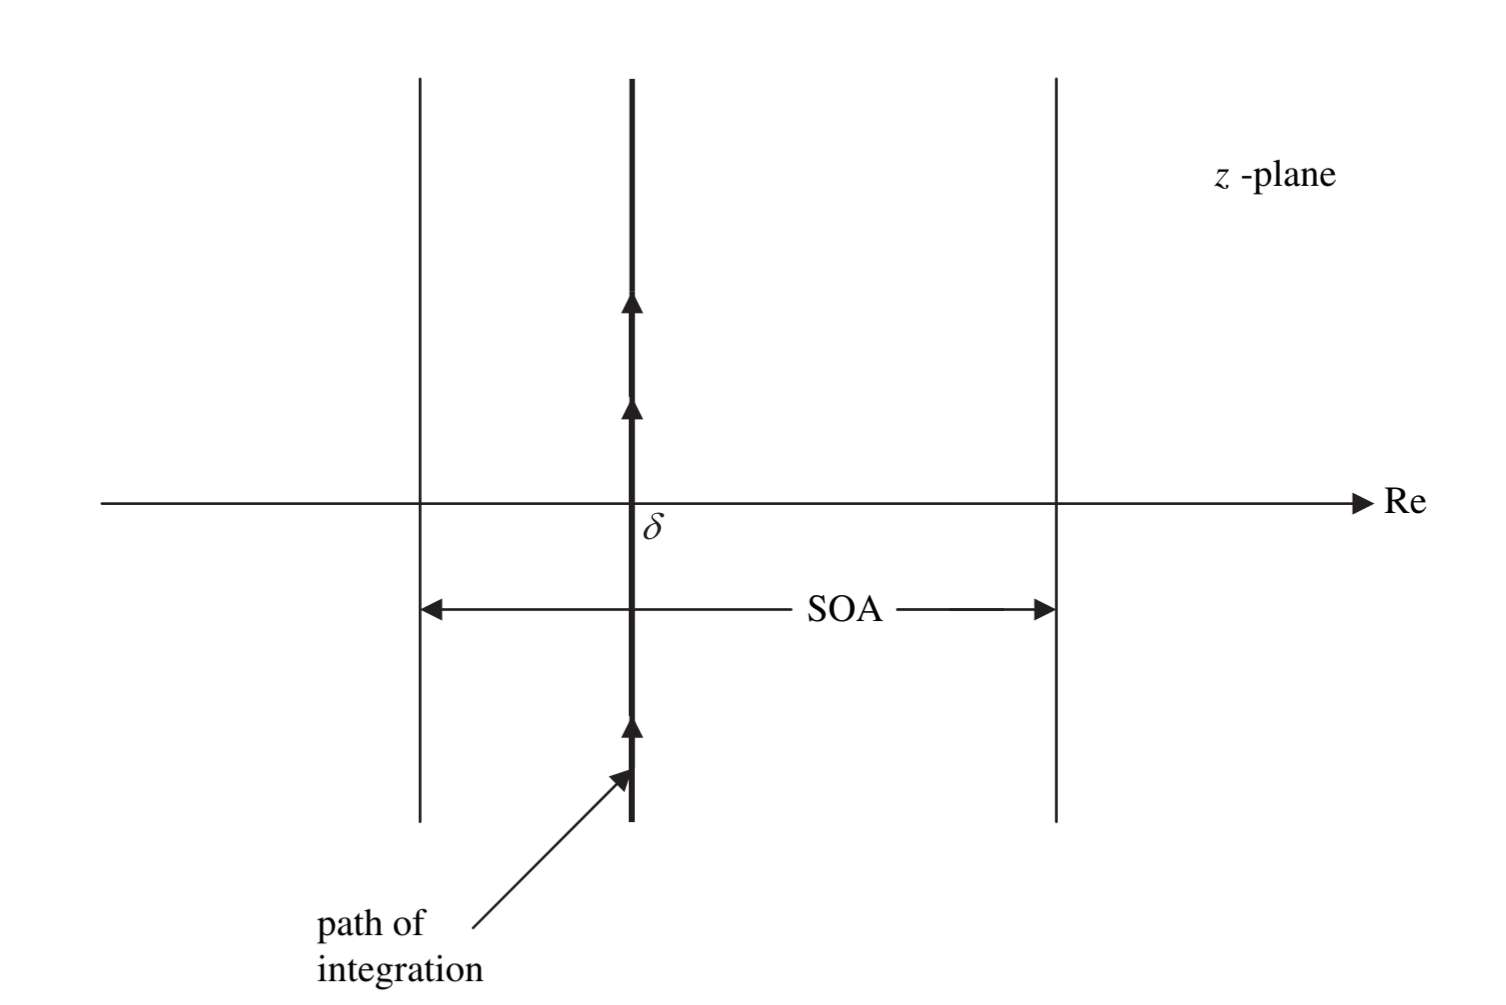
\includegraphics[width=.5\textwidth]{papers/mellin/images/mellin_z}
    \caption{Integrationspfad der Rücktransformation in der $z$-Ebene}
    \label{fig:mellin:z}
\end{figure}
Dies erinnert stark an den Laplaceraum, dessen Variable ebenfalls komplex 
ist und meist in einer Halbebene der komplexen Zahlenebene ab einem 
gewissen Wert $\delta_0$ für den Realteil existiert.
Bei der Rücktransformation muss allerdings der Realteil 
$\delta \in \text{SOA}$ fixiert werden. 
Integriert wird daraufhin über die Parallele der imaginäre Achse an der 
Stelle von $\delta$, wie dargestellt in Abbildung \ref{fig:mellin:z}.

\begin{equation}
    f(x) = 
    \frac{1}{2\pi j} 
    \int\limits_{\delta -j\infty}^{\delta +j\infty} 
    x^{-z} \hat{f}(z) \,\mathrm{d}z
    \label{mellin:mellininv}
\end{equation}
Somit vervollständigt sich das Bild der Mellin-Transformation und fügt 
sich ein in bereits bekannte Integraltransformationen, wie Fourierreihen, 
die Fourier- und Laplacetransformationen sowie deren diskrete Varianten, 
die DFT und z-Transformation.


% Beispiel Skaleninvarianz

